% ==============================================================================
% ================================= Aufgabe 3 =================================
% ==============================================================================

%\chapter{Praktische Umsetzung einer Datengeschichte mit R \textit{(3)}}
%\label{chap:aufgabe3}
%\thispagestyle{fancy}

\section{Praktische Umsetzung einer Datengeschichte mit R \textit{(3)}}

Die Analyse erfolgte in RStudio mit R und den Paketen \texttt{tidyverse}, \texttt{ggplot2}, \texttt{plotly} und \texttt{rmarkdown}.

\refstepcounter{mylisting}
\begin{minipage}[t]{0.48\textwidth}
    \lstinputlisting[
        language={bash},
        style={rstyle},
        firstline=1,
        lastline=4,
        frame=tb,
        numbers=left,
        title=\empty,
    ]{asset/code/Aufgabe3.tex}
\end{minipage}
\hfill
\begin{minipage}[t]{0.48\textwidth}
    \lstinputlisting[
        language={bash},
        style={rstyle},
        firstline=5,
        lastline=7,
        firstnumber=5,
        frame=tb,
        numbers=left,
        title=\empty,
    ]{asset/code/Aufgabe3.tex}
\end{minipage}%
\vspace{-2\baselineskip}%
\captionsetup{hypcap=false}%
\captionof{lstlisting}{Installation der benötigten Software}%
\label{lst:installation}%

\subsection{Szenario und Zielsetzung}
\label{sec:3-einleitung}

Dieses Kapitel widmet sich der praktischen Umsetzung einer datengetriebenen Geschichte zum Klimaschutz. Das Szenario ist einer gemeinnützigen Organisation \textit{(\acs{NGO})} entnommen, die aufzeigen möchte, wie sich \acs{CO2}-Ausstoß und Nutzung erneuerbarer Energien in sechs europäischen Ländern entwickelt haben.

Die zugrundeliegenden Daten sind fiktive Durchschnittswerte für das Jahr 2023 und umfassen die folgenden sechs Länder:

\begin{table}[H]
    \centering
    \begin{tabular}{l c c c}
        \toprule
        \textbf{Land} & \textbf{\acs{CO2} pro Kopf (t)} & \textbf{Erneuerbare (\%)} & \textbf{BIP pro Kopf (€)} \\
        \midrule
        Deutschland  & 8,5 & 47 & 48.000 \\
        Frankreich   & 5,2 & 56 & 44.000 \\
        Polen        & 7,8 & 22 & 32.000 \\
        Spanien      & 6,0 & 51 & 38.000 \\
        Schweden     & 3,9 & 68 & 55.000 \\
        Italien      & 5,9 & 46 & 36.000 \\
        \bottomrule
    \end{tabular}
    \caption{Datengrundlage für die Länderanalyse \textit{(fiktive Werte für 2023)}}
    \label{tab:co2-daten}
\end{table}

Ziel ist es, diese Daten mittels geeigneter Visualisierungen in eine verständliche Geschichte zu überführen. Datenvisualisierung dient nicht nur der Informationsvermittlung, sondern macht komplexe Zusammenhänge auch für ein breites Publikum zugänglich \cite[1]{2}. Für die Umsetzung kommen R und \texttt{ggplot2} zum Einsatz \cite[33]{3}. Die Dokumentation gewährleistet Nachvollziehbarkeit und Reproduzierbarkeit.

% ================================= 3a =================================

\subsection{Erstellung des data.frames \textit{(3a)}}
\label{sec:3a}

Zur Vorbereitung der Mini-Story wird zunächst ein \texttt{data.frame} in R erstellt. Diese Datenstruktur ist für das vorliegende Vorhaben optimal geeignet, da sie heterogene Datentypen, in diesem Fall Zeichenketten \textit{(Strings)} für die Ländernamen und numerische Werte \textit{(Double)} für die Messgrößen, in einer zweidimensionalen tabellarischen Form kombiniert \textit{(\acs{vgl.} \cite[14, 15]{3})}. Gemäß den Konventionen in R wird dabei der Punkt als Dezimaltrennzeichen verwendet \textit{(\acs{vgl.} \cite[46]{3})}.

Der folgende Programmcode nutzt die Funktion \texttt{data.frame()}, um die Werte für das Jahr 2023 konsistent zu organisieren \textit{(\acs{vgl.} \cite[16, 60]{3})}:

\refstepcounter{mylisting}
\begin{minipage}[t]{0.48\textwidth}
    \lstinputlisting[
        language={bash},
        style={rstyle},
        firstline=1,
        lastline=5,
        frame=tb,
        numbers=left,
        title=\empty,
    ]{asset/code/Aufgabe3a.tex}
\end{minipage}
\hfill
\begin{minipage}[t]{0.48\textwidth}
    \lstinputlisting[
        language={bash},
        style={rstyle},
        firstline=6,
        lastline=10,
        firstnumber=6,
        frame=tb,
        numbers=left,
        title=\empty,
    ]{asset/code/Aufgabe3a.tex}
\end{minipage}%
\vspace{-2\baselineskip}%
\captionsetup{hypcap=false}%
\captionof{lstlisting}{Erstellung des data.frames für Aufgabe 3a}%
\label{lst:df-erstellung}%

Die Ausgabe des \texttt{print()}-Befehls zeigt den vollständigen \texttt{data.frame} in tabellarischer Form:

\refstepcounter{mylisting}
\begin{minipage}[t]{0.48\textwidth}
    \lstinputlisting[
        language={R},
        style={rstyle},
        firstline=1,
        lastline=4,
        frame=tb,
        numbers=left,
        title=\empty,
    ]{asset/code/Aufgabe3aII.tex}
\end{minipage}
\hfill
\begin{minipage}[t]{0.48\textwidth}
    \lstinputlisting[
        language={R},
        style={rstyle},
        firstline=5,
        lastline=7,
        firstnumber=5,
        frame=tb,
        numbers=left,
        title=\empty,
    ]{asset/code/Aufgabe3aII.tex}
\end{minipage}%
\vspace{-2\baselineskip}%
\captionsetup{hypcap=false}%
\captionof{lstlisting}{Ausgabe des data.frames}%
\label{lst:df-ausgabe}%

Die Attribute sind gemäß der in Aufgabe 1b definierten \acs{E-Notation} \(E_{6}^{P}(q + n)\) korrekt zugeordnet: \texttt{CO2\_pro\_Kopf}, \texttt{Erneuerbare} und \texttt{BIP\_pro\_Kopf} sind quantitative Merkmale, während \texttt{Land} als nominales Merkmal dient \textit{(\acs{vgl.} \cite[33, 39]{1})}.

% ================================= 3b =================================

\subsection{Visualisierung der erneuerbaren Energien \textit{(3b)}}
\label{sec:3b}

Balkendiagramme eignen sich besonders gut für den Vergleich kategorialer Daten wie Länder, da sie durch die Länge der Balken eine präzise quantitative Interpretation ermöglichen \textit{(\acs{vgl.} \cite[35]{2})}. Um die Lesbarkeit und Ästhetik zu erhöhen, wird das Paket \texttt{ggplot2} verwendet, das eine flexible Gestaltung von Farben und Titeln erlaubt.

Der folgende Code erstellt das geforderte Diagramm mit dem Zuweisungsoperator \texttt{stat = "identity"}, um die tatsächlichen Prozentwerte abzubilden \textit{(\acs{vgl.} \cite[35]{3})}:

\refstepcounter{mylisting}
\begin{minipage}[t]{0.48\textwidth}
    \lstinputlisting[
        language={R},
        style={rstyle},
        firstline=1,
        lastline=9,
        frame=tb,
        numbers=left,
        title=\empty,
    ]{asset/code/Aufgabe3b.tex}
\end{minipage}
\hfill
\begin{minipage}[t]{0.48\textwidth}
    \lstinputlisting[
        language={R},
        style={rstyle},
        firstline=10,
        lastline=18,
        firstnumber=10,
        frame=tb,
        numbers=left,
        title=\empty,
    ]{asset/code/Aufgabe3b.tex}
\end{minipage}%
\vspace{-2\baselineskip}%
\captionsetup{hypcap=false}%
\captionof{lstlisting}{Balkendiagramm der erneuerbaren Energien}%
\label{lst:df-balken}%

Das erzeugte Balkendiagramm ist in Abbildung \ref{fig:balken} dargestellt. Es zeigt, dass Schweden mit 68 \% den höchsten Anteil erneuerbarer Energien aufweist, während Polen mit 22 \% den niedrigsten Anteil hat. Die übrigen Länder – Frankreich \textit{(56 \%),} Spanien \textit{(51 \%)}, Deutschland \textit{(47 \%)} und Italien \textit{(46 \%)} – bewegen sich im Mittelfeld.

\begin{figure}[H]
    \centering
    
\includegraphics[width=0.65\textwidth]{asset/image/Aufgabe3b.png}
    \caption{Nutzung erneuerbarer Energien in ausgewählten Ländern \textit{(2023)}}
    \label{fig:balken}
    \emph{Quelle: Eigene Darstellung}
\end{figure}

% ================================= 3c =================================

\subsection{Scatterplot: \texorpdfstring{\acs{CO2}}{CO2}-Ausstoß \acs{vs.} erneuerbare Energien \texorpdfstring{\textit{(3c)}}{(3c)}}
\label{sec:3c}

Ein Scatterplot \textit{(Streudiagramm)} ist das ideale Instrument, um die Beziehung zwischen zwei metrischen Variablen zu untersuchen und Korrelationen oder Muster sichtbar zu machen. Durch die Positionierung der Datenpunkte im zweidimensionalen Koordinatensystem lässt sich unmittelbar ablesen, wie die Werte der \(x\)-Achse \textit{(erneuerbare Energien)} mit denen der \(y\)-Achse \textit{(\acs{CO2}-Ausstoß)} interagieren. \textit{(\acs{vgl.} \cite[29, 31, 53]{2})}

Der folgende Code erstellt den Scatterplot mit einer Regressionslinie zur Verdeutlichung des Trends: \pagebreak[3]

\refstepcounter{mylisting}
\begin{minipage}[t]{0.48\textwidth}
    \lstinputlisting[
        language={R},
        style={rstyle},
        firstline=1,
        lastline=9,
        frame=tb,
        numbers=left,
        title=\empty,
    ]{asset/code/Aufgabe3c.tex}
\end{minipage}
\hfill
\begin{minipage}[t]{0.48\textwidth}
    \lstinputlisting[
        language={R},
        style={rstyle},
        firstline=10,
        lastline=18,
        firstnumber=10,
        frame=tb,
        numbers=left,
        title=\empty,
    ]{asset/code/Aufgabe3c.tex}
\end{minipage}%
\vspace{-2\baselineskip}%
\captionsetup{hypcap=false}%
\captionof{lstlisting}{Scatterplot mit Regressionslinie}%
\label{lst:df-scatter}%

Das in Abbildung \ref{fig:scatter} dargestellte Streudiagramm zeigt einen negativen Zusammenhang zwischen dem Anteil erneuerbarer Energien und dem \acs{CO2}-Ausstoß pro Kopf. Länder mit einem höheren Anteil erneuerbarer Energien, wie Schweden \textit{(68 \%)}, weisen tendenziell niedrigere \acs{CO2}-Emissionen pro Kopf auf \textit{(3,9 Tonnen)}, während Länder mit einem geringeren Anteil – wie Polen \textit{(22 \%)}, höhere Emissionen verzeichnen \textit{(7,8 Tonnen)}. Die eingezeichnete Regressionsgerade bestätigt diesen negativen Trend, wobei die Streuung der Datenpunkte auf weitere Einflussfaktoren hindeutet.

Interpretation des Musters: Es ist ein deutlicher negativer Zusammenhang erkennbar: Je höher der Anteil erneuerbarer Energien in einem Land ist, desto geringer fällt tendenziell der \acs{CO2}-Ausstoß pro Kopf aus.

\begin{figure}[H]
    \centering
    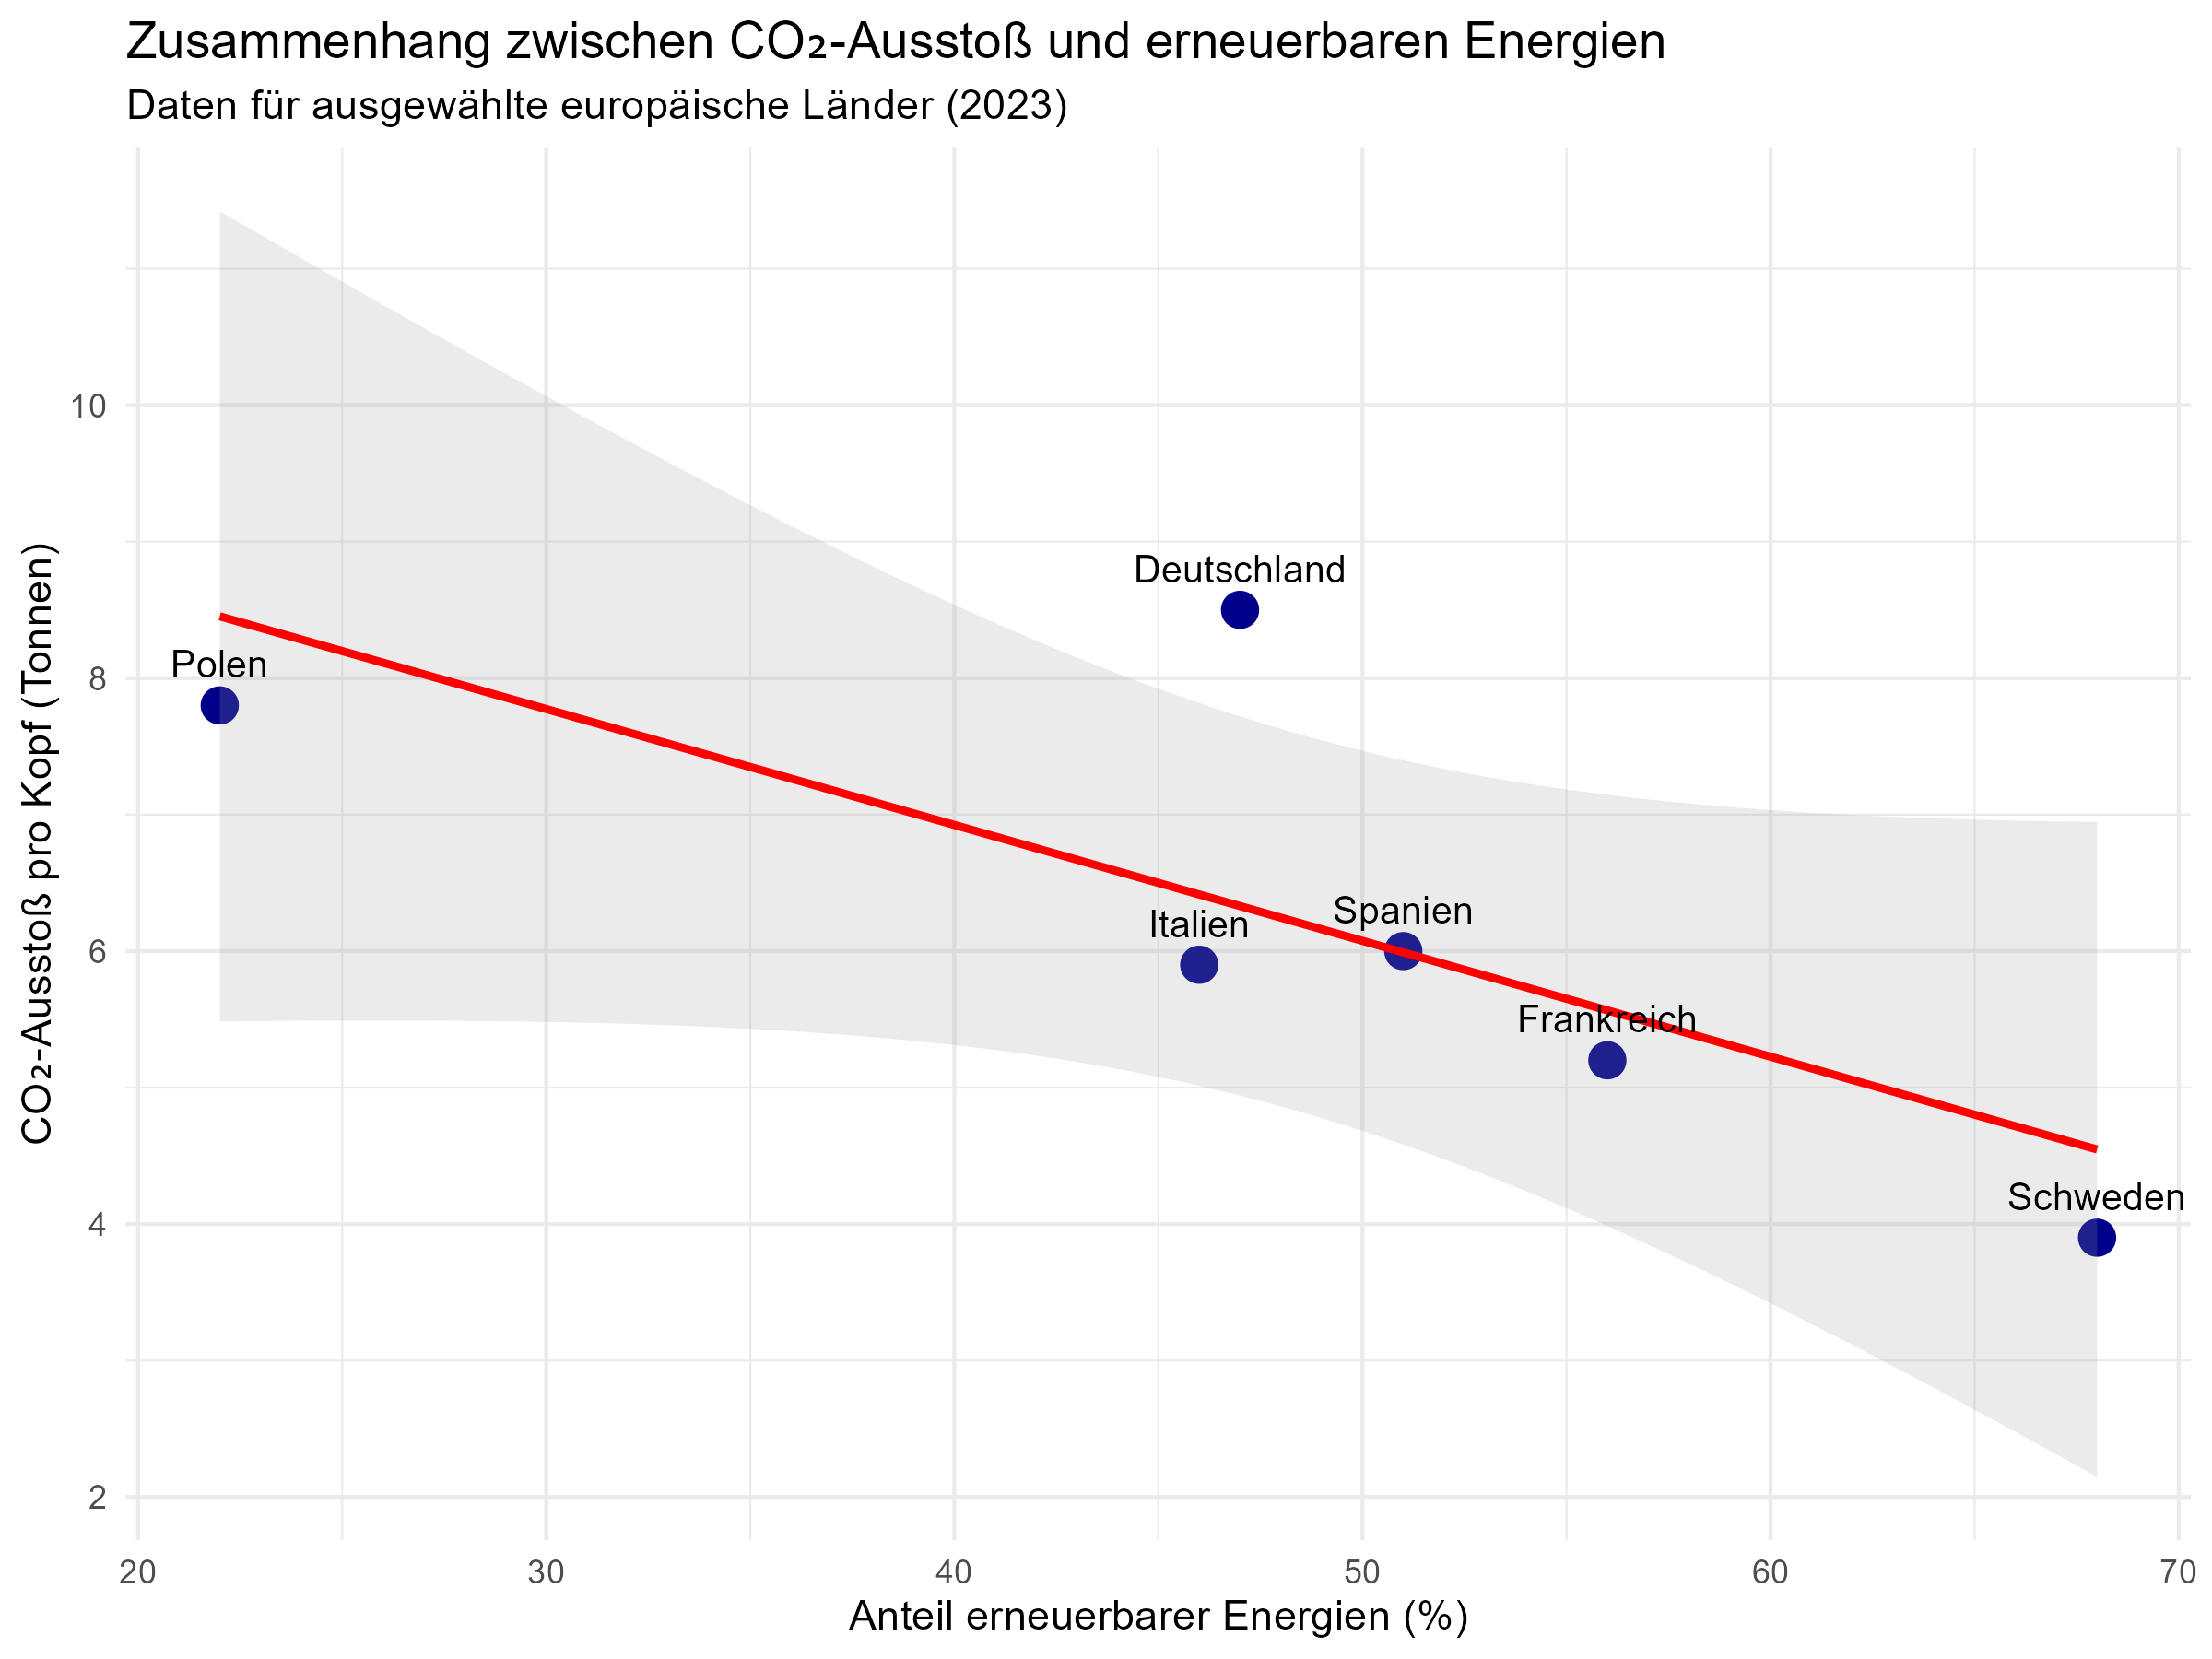
\includegraphics[width=0.70\textwidth]{asset/image/Aufgabe3c.png}
    \caption{\acs{CO2}-Ausstoß pro Kopf \acs{vs.} Anteil erneuerbarer Energien}
    \label{fig:scatter}
    \emph{Quelle: Eigene Darstellung}
\end{figure}

% ================================= 3d =================================

\subsection{Mini-Story für ein Laienpublikum \textit{(3d)}}
\label{sec:3d}

Auf Grundlage der erstellten Visualisierungen lässt sich folgende Geschichte für ein Laienpublikum formulieren:

\begin{quote}
\itshape
Die Analyse der Daten für das Jahr 2023 verdeutlicht den entscheidenden Einfluss der Energiewende auf den persönlichen \acs{CO2}-Fußabdruck in Europa. Als klarer Vorreiter positioniert sich Schweden, das mit einem Anteil von 68 \% erneuerbarer Energien den geringsten \acs{CO2}-Ausstoß pro Kopf erzielt. Im Gegensatz dazu weist Polen mit nur 22 \% Grünstrom-Anteil einen hohen Emissionswert auf, was einen dringenden Handlungsbedarf signalisiert. Der beobachtete negative Zusammenhang bestätigt dabei die wissenschaftliche Erkenntnis: Je konsequenter ein Land auf regenerative Quellen setzt, desto effektiver sinken tendenziell die schädlichen Pro-Kopf-Emissionen. Deutschland belegt mit 47 \% Erneuerbaren einen mittleren Platz, muss jedoch seine Anstrengungen weiter intensivieren, um zu den ökologischen Spitzenreitern aufzuschließen. Diese Ergebnisse unterstreichen für die Öffentlichkeit, dass der massive Ausbau grüner Energien der zentrale Hebel für einen wirksamen und messbaren Klimaschutz ist \textit{(\acs{vgl.} \cite[44-46, 70, 67]{2})}.
\end{quote}

% ================================= 3e =================================

\subsection{Export als RMarkdown-Report \textit{(3e)}}
\label{sec:3e}

Der Export der erarbeiteten Story erfolgt mithilfe von R Markdown, was eine nahtlose Kombination aus erklärendem Text, ausführbarem Programmcode und den daraus resultierenden Visualisierungen in einem einzigen, reproduzierbaren Dokument ermöglicht. \citeauthor{3} beschreibt diese Arbeitsweise als einen der zentralen Vorteile von R Markdown, da sie die Nachvollziehbarkeit und Dokumentation von Analysen erheblich vereinfacht \cite[55-59]{3}.

\subsubsection{Aufbau und Erstellung des RMarkdown-Dokuments}

Der Export erfolgte mit R Markdown, das erklärenden Text, Code und Visualisierungen in einem reproduzierbaren Dokument vereint \cite[55-59]{3}. Ein RMarkdown-Dokument gliedert sich in drei Bestandteile: \texttt{YAML}-Kopfzeile \textit{(Metadaten)}, narrativen Text und R-Codeblöcke \textit{(Chunks)}. Die \texttt{.Rmd}-Datei wurde in RStudio über \texttt{File → New File → R Markdown} erstellt.

\refstepcounter{mylisting}
\begin{minipage}[t]{0.48\textwidth}
    \lstinputlisting[
        language={R},
        style={rstyle},
        firstline=1,
        lastline=33,
        frame=tb,
        numbers=left,
        title=\empty,
    ]{asset/code/Aufgabe3e.tex}
\end{minipage}
\hfill
\begin{minipage}[t]{0.48\textwidth}
    \lstinputlisting[
        language={R},
        style={rstyle},
        firstline=34,
        lastline=64,
        firstnumber=34,
        frame=tb,
        numbers=left,
        title=\empty,
    ]{asset/code/Aufgabe3e.tex}
\end{minipage}%
\vspace{-2\baselineskip}%
\captionsetup{hypcap=false}%
\captionof{lstlisting}{RMarkdown-Code für den Report}%
\label{lst:df-rmd}%

\subsubsection{Export des Reports}

Der eigentliche Exportvorgang \textit{(Rendering)} wird anschließend entweder über die Schaltfläche \texttt{Knit} in der Menüleiste von RStudio oder über den Befehl \texttt{rmarkdown::render()} in der Konsole angestoßen:

\begin{lstlisting}[language=R, style=rstyle, caption=Export des RMarkdown-Reports, label=lst:rmd-render]
rmarkdown::render("co2\_analyse.Rmd", output\_format = "html\_document")
\end{lstlisting}

Durch die Angabe von \texttt{output\_format = "html\_document"} wird ein interaktiver \acs{HTML}-Report erzeugt, der direkt im Webbrowser betrachtet werden kann. Während interaktive \acs{HTML}-Berichte direkt im Webbrowser betrachtet werden können, erfordert der Export in das \acs{PDF}-Format zusätzlich eine lokale Installation des Textsatzsystems LaTeX:

\begin{lstlisting}[language=R, style=rstyle, caption=Export als \acs{PDF}, label=lst:rmd-pdf]
rmarkdown::render("co2_analyse.Rmd", output_format = "pdf_document")
\end{lstlisting}

\begin{notice}
Die Erstellung eines \acs{PDF}-Dokuments setzt eine LaTeX-Installation voraus.
\end{notice}

% ========================== RMarkdown-Report Inhalt ===========================

% ==============================================================================
% ================================= Aufgabe 3 =================================
% ==============================================================================